\section{Overview}
Smokeview uses OpenGL to visualizing fire and smoke data.  OpenGL
is a 3D graphics library used to specify the location, color and
lighting of objects residing within a ``3D world'' defined by FDS,
the Fire Dynamics Simulator. In the context of FDS, these objects
may be used to represent geometry such as blockages or to
visualize data. Smokeview visualizes data as tracer particles, 2D
shaded contours or 3D level iso-surfaces {\em etc.}  Soot data or
smoke may also be visualized using a variation of a 2D shaded
contour where transparency rather than color is used to represent
the opacity or optical thickness of smoke.

A detailed description of OpenGL and how it may be used to
visualize objects and data is given in references
\cite{OpenGLRed,SUPERBIBLE}. The following is a short summary of
how Smokeview uses OpenGL to visualize fire and smoke data.

\begin{figure}[t]
\begin{center}
\includegraphics[width=3.5in]{figurest/shapes}
\end{center}
\caption[Points, lines and a shaded triangle drawn using OpenGL.]
{Points, lines and a shaded triangle drawn using OpenGL. Vertices
are defined using {\tt glVertex*} and the particular shapes are
generated by passing {\tt GL\_POINTS}, {\tt GL\_LINES}, and {\tt
GL\_TRIANGLE}\ to {\tt glBegin()} } \label{figshapes}
\end{figure}
\subsection{Objects} The fundamental object in OpenGL is a
vertex. An OpenGL vertex has the same meaning as in geometry, a
three dimensional location. A vertex is specified using {\bf
glVertex*()}\ where in Smokeview * is usually 3f meaning that
three floating point scalar values are specified. Smokeview also
uses {\bf 3fv}, allowing one to pass a pointer to data ({\em
i.e.}\ a vector) which is more efficient. To specify a vertex at
$(0,1,2)$ one would use (in C)
\begin{verbatim}
glVertex3f(0.0,1.0,2.0);
\end{verbatim}
Various geometric objects, as illustrated in Figure
\ref{figshapes}, may be specified by grouping vertices together
and surrounding them with calls to {\tt glBegin()}\ and {\tt
glEnd()}. To draw a shaded triangle one would use
\begin{verbatim}
glBegin(GL_TRIANGLE);
glVertex3f(0.0,0.0,0.0);
glVertex3f(0.0,1.0,0.0);
glVertex3f(1.0,0.0,0.0);
glEnd();
\end{verbatim}
To draw points or to connect the vertices with lines (also shown
in Figure \ref{figshapes}) one would replace {\tt GL\_TRIANGLE}\
with {\tt GL\_POINTS}\ or {\tt GL\_LINES}\ respectively.

\begin{figure}[t]
\begin{center}
\begin{tabular}{cc}
\includegraphics[width=2.5in]{figurest/th_transparent}&
\includegraphics[width=2.5in]{figurest/th_solid}\\
transparent&solid\\
\end{tabular}
\end{center}
\caption {A slice file drawn transparently mixes or blends the
slice colors with those in the background.  When drawn opaquely,
any portion of the scene behind the slice file is hidden. }
\label{figtransparent}
\end{figure}

Triangles are the fundamental constructs Smokeview uses to
visualize objects.  To be useful though these objects need to be
colored, moved and projected onto a 2D terminal screen. These
topics are discussed in the following sections.
\subsection{Color} Besides location, a vertex also has an attribute of color.
Color in OpenGL consists of four components, red, green, blue, and
alpha. Each component ranges from 0.0 to 1.0. The alpha component
represents opaqueness, 0.0 being completely transparent and 1.0
being completely opaque. Smokeview uses the alpha parameter to
blend the currently drawn object with the background where the
background is the accumulation of all objects drawn to that point.
Choosing an alpha smaller than one (and not zero) allows one to
``see through'' an object. Slice files as illustrated in Figure
\ref{figtransparent}, are drawn using transparency. Data chopping
or hiding data in Smokeview slice files is also implemented using
blending or transparency. Data to be hidden is given an alpha
value of 0.0 causing it to be completely transparent.

Complications arise because the blending model in OpenGL is
neither commutative nor associative. The order objects are drawn
is significant.  In order to prevent inconsistent drawing, opaque
objects must be drawn first then partially transparent objects
must be drawn next from back to front (from the point of view of
the observer). Otherwise transparent objects may appear blended in
front of objects when they should in fact be obscured.

When lighting is not applied, colors within a triangle are
determined in two steps using bi-linear interpolation. First,
colors along a triangle edge are linearly interpolated using the
two colors of the vertices bounding the edge. Second, the interior
colors are determined along a horizontal scan line again using
linear interpolation using colors previously interpolated on the
triangle edge.

Flat shaded triangles may be drawn more efficiently but are not
effective at visualizing a 3D effect.  More sophisticated shading
techniques are required and are discussed next.

\begin{figure}[t]
\begin{center}
\begin{tabular}{cc}
\includegraphics[width=2.5in]{figurest/th_unlit}&\includegraphics[width=2.5in]{figurest/th_lit}\\
flat shading&smooth (Gouraud) shading\\
\end{tabular}
\end{center}
\caption [The FDS townhouse case drawn using flat and smooth
shading.] { The FDS townhouse case drawn using flat and smooth
shading. All blockage surfaces have identical colors when drawn
with flat shading.  When drawn with smooth shading, blockage
colors change.  Surfaces are darker when not in direct view of the
light source adding to a sense of depth. } \label{figlighting}
\end{figure}

\begin{figure}[t]
\begin{center}
\begin{tabular}{cc}
\includegraphics[width=2.5in]{figurest/triangle_normal}&\includegraphics[width=2.5in]{figurest/triangle_normal2}\\
\includegraphics[width=2.5in]{figurest/sphere_facet}&\includegraphics[width=2.5in]{figurest/sphere_lit}\\
separate normals $\rightarrow$ faceted drawing&averaged normals $\rightarrow$ smooth drawing\\
\end{tabular}
\end{center}
\caption {Two sphere drawn showing the effect of using averaged
normals.  Using non-averaged normals results in a faceted or
gem-like appearance. } \label{fignormals}
\end{figure}

\subsection{Lighting} OpenGL uses two shading methods for
drawing objects, flat and Gouraud shading.  Gouraud shading is
also referred to as smooth shading.  Flat shading assumes that
objects are drawn in an environment with uniform lighting - light
surrounds an object equally in all directions. Smooth lighting on
the other hand assumes that light comes from a particular
direction.  This causes subtle changes in color to occur across an
object's surface. Figure \ref{figlighting} shows examples of FDS
blockages (the standard townhouse scenario) drawn using flat and
smooth shading. Flat shading obscures the three dimensionality of
the scene.

A normal vector, another vertex attribute, is required to
implement a smooth lighting scheme. A normal vector points in a
direction perpendicular to the surface at the vertex. OpenGL uses
this information to estimate the fraction of light from the light
source reflected off of the given surface and intercepted by the
observer.  This is similar to a configuration factor calculation
performed in fire modelling.  The amount of light perceived by the
observer depends on the relative orientation of the light source,
the object (as specified by the location and normal vector of each
vertex) and the observer.

For planar surfaces, the same normal vector is applied to each
vertex defining the surface. For curved surfaces, normal vectors
are determined using an average of the normal directions of faces
surrounding the vertex.  If normals are not averaged then the
discontinuity in slope going from one face or triangle to another
will result in a faceted or gem-like appearance.  Figure
\ref{fignormals} shows examples of drawing using non-averaged and
averaged normals.

The Gouraud method for shading then determines a vertex color
using the angle between the light source direction and the vertex
normal vector. The color of the object being shaded is then
determined by interpolating these colors.

Smokeview uses smooth shading or lighting to draw blockages and
iso-surfaces. Particle, slice and boundary files are drawn without
shading as are 3D smoke and Plot3D files.



\subsection{Movement} One would like to manipulate objects.  This process can be thought
of in two equivalent ways - keeping the scene fixed and changing
the observer's location and view direction or keeping the observer
fixed and moving, rotating and/or scaling the scene.

Objects are moved mathematically in OpenGL by multiplying the
object's vertices (a vector) with the current OpenGL {\bf
modelview}\ matrix.  This multiplication is usually performed in
hardware by the video card.  The modelview matrix is initialized
to the identity matrix then multiplied by matrices representing
translation, rotation or scaling as as the scene is moved using
the {\tt glTranslate}, {\tt glRotate}\ and {\tt glScale} OpenGL
calls.

OpenGL uses what are called homogenous coordinates meaning that
the $(x,y,z)$ coordinate is represented as $(x,y,z,w)$ where in
Smokeview $w=1$.  A translation by $(x,y,z)$ is performed using
{\tt glTranslate3f(x,y,z)} which causes the matrix
\begin{eqnarray*}
T=\left(%
\begin{array}{cccc}
  1 & 0 & 0 & -x \\
  0 & 1 & 0 & -y \\
  0 & 0 & 1 & -z \\
  0 & 0 & 0 & 1 \\
\end{array}%
\right)
\end{eqnarray*}
to be applied to the modelview matrix.  A rotation of $\theta$
degrees about an axis along the unit-vector $(u,v,w)$ is performed
using {\tt glTranslate3f(u,v,w,$\theta$)}.  A rotation of $\theta$
degrees about the $x$ axis is performed using {\tt
glTranslate3f(1.0,0.0,0.0,$\theta$)} which causes the matrix

\begin{eqnarray*}
R=\left(%
\begin{array}{cccc}
  1 & 0 & 0 & 0 \\
  0 & \cos(\theta) & -\sin(\theta) & 0 \\
  0 & \sin(\theta) & \cos(\theta) & 0 \\
  0 & 0 & 0 & 1 \\
\end{array}%
\right)
\end{eqnarray*}
to be applied to the modelview matrix.  A scaling by $u$, $v$ $w$
along the $x$, $y$ and $z$ axese respectively is performed using
{\tt glScale3f(u,v,w)} which causes the matrix
\begin{eqnarray*}
S=\left(%
\begin{array}{cccc}
  u & 0 & 0 & 0 \\
  0 & v & 0 & 0 \\
  0 & 0 & w & 0 \\
  0 & 0 & 0 & 1 \\
\end{array}%
\right)
\end{eqnarray*}
to be applied to the modelview matrix.  Smokeview uses scaling to
view cases with large aspect ratios, tunnel fires for example.

The desired translation and rotation amounts are communicated
between the user and Smokeview using keyboard and/or mouse
callback routines.  Mouse motion is intercepted by the GLUT
library routine (see section \ref{sect_glut}) and converted from
screen pixel coordinates to translation or rotation amounts.


\subsection{Projection and Viewports}
\begin{figure}[t]
\begin{center}
\begin{tabular}{cc}
\includegraphics[width=2.75in]{figurest/figviewport}&
\includegraphics[width=2.75in]{figurest/figviewport2}\\
screen viewport $\leftarrow$ 3D scene&
Smokeview viewports\\
\end{tabular}
\end{center}
\caption{Example view frustum used to convert 3D scenes to 2D
screen viewports.}
 \label{figviewports}
\end{figure}
The next step in the drawing process is to flatten or project the
3D scene onto the 2D terminal screen where it will be viewed. A
viewport is the particular portion of the screen where the drawing
is to occur.  Smokeview defines separate viewports for drawing the
title, time bar, color bar and the 3D scene.  Figure
\ref{figviewports} illustrates the relationship between the 3D
scene and the 2D screen giving examples of viewports used by
Smokeview. Two common schemes for projecting geometry from 3D to
2D  are orthographic and perspective. An orthographic projection
is size preserving. Objects in the foreground take up the same
amount of screen space as objects in the background. A perspective
projection causes objects to take up less screen space when they
are drawn in the background resulting in the illusion of depth or
perspective, hence its name. Both projection methods are available
in Smokeview.

Smokeview uses {\tt glFrustum}\ to perform perspective projections
\begin{verbatim}
      glFrustum(
        (double)fleft,(double)fright,
        (double)fdown,(double)fup,
        (double)fnear,(double)ffar);
\end{verbatim}
and {\tt glOrtho}\ to perform orthographic projections
\begin{verbatim}
      glOrtho(
        (double)fleft,(double)fright,
        (double)fdown,(double)fup,
        (double)fnear,(double)ffar);
\end{verbatim}

where {\tt fleft}, {\tt fright}, {\tt fdown}, {\tt fup}, {\tt
fnear}, {\tt ffar} are six clipping planes bounding the view
frustum (truncated pyramid) for the perspective projection or the
box in the orthographic projection.  Drawing does not occur
outside of the 3D region defined by these 6 clipping planes. An
additional six clipping planes parallel to the x, y and z axes may
be activated in Smokeview (using the clipping dialog box) to hide
geometry making it easier to see interior objects or
visualizations.  OpenGL allows one to define clipping planes along
arbitrarily oriented planes.



\subsection{Graphics Library Utility Toolkit - GLUT}
OpenGL draws the 3D geometry but does not interact with the user
or the operating system. Smokeview uses the graphics library
utility toolkit (GLUT) for interacting with the user {\em via}\
the keyboard and mouse and for interacting with the operating
system to swap display buffers, to display fonts, to set maximum
frame rates {\em etc}. Though not as sophisticated as other
libraries, GLUT is simple to use and is portable allowing
Smokeview to be built on a number of different computer platforms
including a PC running Windows or Linux, a Silicon Graphics
workstation running IRIX or a Macintosh running OSX.

\paragraph{Buffers} Smokeview uses several buffers provided by
OpenGL for visualization.  GLUT is used to manipulate these
buffers. Smokeview uses double buffering.  Drawing occurs in the
{\bf back buffer}\ while simultaneously the scene is displayed in
the {\bf front buffer}. Smokeview uses the GLUT routine {\tt
glutSwapBuffers();}\ to swap the front and back buffers once
drawing is complete. Screen flickering would occur if drawing and
display used the same buffer.

Hidden lines and surfaces are removed from a scene using the {\bf
depth buffer}.  Each time Smokeview draws an object, its depth
(distance from the observer) is compared to the value previously
stored in the depth buffer.  If the object's depth is less than
the value stored in the depth buffer then the object is considered
visible and the new depth value is store in the buffer. Otherwise
the depth buffer remains unchanged and the object is considered
hidden.

\paragraph{Initialization and Callback Routines}
Initializations are performed by GLUT to set up windows and to
define display modes.  Smokeview defines the display to handle
color, a depth buffer and double buffering by passing the OpenGL
keywords {\tt GLUT\_RGB}, {\tt GLUT\_DEPTH} and {\tt GLUT\_DOUBLE}
to {\tt glutInitDisplayMode} as in

\begin{verbatim}
  glutInitDisplayMode(GLUT_RGB|GLUT_DEPTH|GLUT_DOUBLE);
\end{verbatim}

Smokeview creates a window with width {\tt windW}\ and height {\tt
windH} using the GLUT calls

\begin{verbatim}
  glutInitWindowSize(windW, windH);
  glutCreateWindow("");
\end{verbatim}

and defines callbacks with

\begin{verbatim}
  glutSpecialUpFunc(specialkeyboard_up);
  glutKeyboardUpFunc(keyboard_up);
  glutKeyboardFunc(keyboard);
  glutMouseFunc(mouse);
  glutSpecialFunc(specialkeyboard);
  glutMotionFunc(motion);
  glutReshapeFunc(Reshape);
  glutDisplayFunc(Display);
\end{verbatim}

A callback is a routine that is called when a particular event
occurs.  For Smokeview these events would be when a keyboard key
is depressed (or when the key is released), when the mouse is
clicked or when the mouse is moved.  Smokeview determines rotation
and translation amounts using the {\tt motion} callback defined
with {\tt glutMotionFunc(motion)}.

%
% .............. new section ..............................
%
\section{Visualizing Smoke Realistically}

Smokeview uses several methods for visualizing fire and smoke
data.  These methods range from tracer particles, 2D animated
shaded contours and 3D iso-surfaces to realistic techniques using
volumetric methods. Smokeview performs these visualizations using
prediction data simulated by the Fire Dynamics Simulator (FDS) in
particular soot density data at each grid cell at each time step.

The smoke visualization procedure can be summarized as follows.
The computations are split into two parts. FDS computes the flow
and density of soot throughout the computational domain.  It then
computes opacity values in the x direction at each grid node.
These opacity values are then compressed and saved to a file for
use by Smokeview. Smokeview then reads and corrects these values
according to the particular view direction or grid plane skipping
implemented. Each plane is colored black with opaqueness or alpha
values assigned according the soot densities provided by the fire
model (using Beer's law). The alpha values are corrected according
to the view direction and the graphics hardware combines or
composites the planes together forming one image. The steps for
computing and drawing smoke are outlined in Figure
\ref{figflowchart}.

\begin{figure}[t]
\begin{center}
\begin{tabular}{cc}
\includegraphics[width=2.5in]{figurest/flowchartpdf_fds}&\includegraphics[width=2.5in]{figurest/flowchartpdf_smokeview}\\
FDS pre-computations&Smokeview computations and corrections\\
\end{tabular}
\end{center}
\caption [Flowchart of FDS and Smokeview computations for
visualization smoke realistically.] {Flowchart of FDS and
Smokeview computations for visualization smoke realistically. FDS
computes obscuration parameters from one grid plane to the next.
Smokeview corrects these parameters to account for non-axis
aligned view directions.} \label{figflowchart}
\end{figure}

\begin{figure}[t]
\begin{center}
\includegraphics[width=3.5in]{figurest/smoke_setup}
\end{center}
\caption {Smoke is drawn by blending the smoke color with the
background color.  The amount of blending depends on the amount of
obscuration as determined from soot density and path length.}
\label{figsmokesetup}
\end{figure}

\begin{figure}[t]
\begin{center}
\begin{tabular}{cc}
\includegraphics[width=2.5in]{figurest/th_smoke_side}&\includegraphics[width=2.5in]{figurest/th_smoke_front}\\
side view&front view\\
\end{tabular}
\end{center}
\caption{Side and front view of partially transparent planes used
in smoke visualization.} \label{figthsmoke}
\end{figure}

To draw the smoke, Smokeview blends the smoke color (black) with
the background color.  The amount of blending depends on the
integrated smoke thickness along a line of sight between the
observer's ``eye'' and the observation point. This is illustrated
in Figure \ref{figsmokesetup}. This integration is performed using
the video hardware to display and then combine a series parallel
planes. Figure \ref{figthsmoke} shows two parallel smoke planes as
normally viewed from the front and also from the side to make the
separate planes visible. Figure \ref{figplume} shows four plume
image, illustrating how the smoke looks more realistic as more
smoke planes are included in the image.

Realistic smoke visualization makes Smokeview a more suitable tool
for fire fighting training applications.  The trainee can better
experience and react to the fire. These visualization techniques
are a challenge however to implement. The storage requirements for
describing smoke can easily exceed the disk capacities of present
operating systems. For, unlike slice and PLOT3D files, data is
required at all grid nodes and at all times steps (rather than on
a single plane at all time steps in the case of slice files or at
all grid nodes at one time step in the case of PLOT3D files). The
computation required both by the CPU and the video card to display
each frame can easily exceed even 0.1 seconds, the time
corresponding to a 10 frame per second display rate.  The physics
required to describe smoke and its interactions with itself and
surrounding light sources is complex and computationally
intensive. Approximations and simplifications are clearly
required.  The following sections describe the techniques and
approximations Smokeview uses to visualize smoke and fire
realistically.


\begin{figure}[t]
\begin{center}
\begin{tabular}{cc}
\includegraphics[width=2.5in]{figurest/splume_20_27}&\includegraphics[width=2.5in]{figurest/splume_17_27}\\
slices 20 to 27&slices 17 to 27\\
\includegraphics[width=2.5in]{figurest/splume_14_27}&\includegraphics[width=2.5in]{figurest/splume_11_27}\\
slices 14 to 27&slices 11 to 27
\end{tabular}
\end{center}
\caption [Smoke plume visualized using several vertical parallel
partially transparent planes.] {Smoke plume visualized using
several vertical parallel partially transparent planes. The
transparency is computing using soot density which is in turn
computed using conservation equations for mass, momentum and
energy. } \label{figplume}
\end{figure}

\paragraph{Literature Review}

\cite{stam:99}\cite{stam:95}\cite{fedkiw:01}\cite{stam:00}
\cite{PRESS88a} \cite{marchingcubes}

\cite{stam:99a}\cite{sayood:96a}\cite{Bajaj:01a}\cite{Levoy:90a}
\cite{Sabella:88a}\cite{Gardner:85a}

\subsection{Computing Smoke Obscuration}
\subsubsection{Smoke Flow Model}
 \label{section:firemodel}


Smokeview visualizes 3D smoke using soot density data simulated by
the Fire Dynamics Simulator (FDS)\cite{FDS_Tech_Guide_4}.  FDS, is
a computational fluid dynamics model (CFD) using equations for the
conservation of mass, an approximate form of the Navier-Stokes
equation (Newton's 2nd law or conservation of momentum)
appropriate when flow velocities are less than 30 \% the speed of
sound and the conservation of energy (first law of
thermodynamics). The approximations used in FDS involve the
filtering out of acoustic waves while allowing for large
variations in temperature and density\cite{Rehm:1}.  Efficient
techniques for solving these are equations are described in
Refs.\cite{McGrattan:1,Baum:1}. FDS uses a form of CFD known as
large eddy simulation (LES) to predict the thermal conditions
resulting from a compartment fire. LES is a way of describing the
effect of turbulence on the flow field. Turbulence is a phenomena
that causes gases to mix over a wide range of length scales making
it hard to replicate with even the fastest computers. The
realistic smoke visualization techniques discussed here are needed
for interpreting the massive amounts of data generated by FDS.

The fire itself is a source term in the governing equations,
creating buoyant motion that drives the smoke and hot gases
throughout the room. The chemistry of the combustion process is
complicated by the fact that the fuel for the fire may include
room furnishings, ceiling materials, wall and floor coverings,
i.e. a wide assortment of different materials. FDS makes
simplifications about the combustion, essentially saying that fuel
and oxygen burn readily when mixed. The rate at which energy is
generated is obtained from experiments. There is no attempt to
model the fundamental chemistry which can involve hundreds of
chemical reactions.

The modeling equations are solved by discretizing all spatial
derivatives using second order finite differences. The flow
variables are updated in time using an explicit second order
predictor-corrector scheme.  First in the predictor step the
solution variables are estimated at the next time step and the
pressure is estimated using a Poisson equation solved using an FFT
based Fast Poisson solver\cite{Sweet:1}. The time step is bounded
to ensure that flow does not cross more then one grid cell in a
time step to enforce a stability condition . The solution
variables are then corrected using the computed pressure. The flow
velocities are then corrected using the corrected pressure.  The
use of rectangular grids allow the use of a fast direct
(non-iterative) Poisson solver in FDS resulting in more efficient
solutions.



\subsubsection{Computing Alphas From Soot Density} The obscuration
or fraction of light absorbed by a medium may be computed using
Beer's law\cite{Siegel:2001}. Beer's law is an empirical
relationship relating light absorption to the material properties
of the media the light is travelling through, in this case the
density of soot.

Let $\Delta x$ be the distance between two nodes as illustrated in
Figure \ref{figAlpha}.  Let $k$ be the mass extinction coefficient
(proportionality constant relating soot density and absorption)
and $s_i$ be the density of soot along a ray between two planes at
node $i$.  Then the obscuration, $\alpha_i$, at node $i$ is given
by
\begin{equation}
\alpha_i=1-\exp(-k\Delta xs_i) \label{eq:alpha}
\end{equation}

\begin{figure}[t]
\centerline{\includegraphics[width=4.5in]{figurest/figAlpha}}
\caption [Opaqueness is computed using the soot density, the mass
extinction coefficient and the distance to the next set of
nodes.]{ The opaqueness parameter, $\alpha$, at node $i$ is
computing using the soot density, $s_i$, the mass extinction
coefficient, $k$ and the distance between sets of nodes, $\Delta
x$. } \label{figAlpha}
\end{figure}

\subsubsection{Adjusting the Absorption Parameter}

\begin{figure}[t]
\centerline{\includegraphics[width=4.5in]{figurest/figray}}
\caption [Diagram illustrating the adjustment needed to opaqueness
parameter, $\alpha$, for non axis aligned views.] { Diagram
illustrating adjustment needed to opaqueness parameter, $\alpha$,
for non axis aligned views. The $\alpha$ value along the ray
containing the $\hat{x}$ segment needs to be larger to account for
the longer path length. } \label{figray}
\end{figure}
The absorption parameter, $\alpha$ needs to be adjusted when
either
\begin{enumerate}
\item the view direction is not aligned along the axis orthogonal
to the viewing planes (as in Figure \ref{figray}, \item the
distance between adjacent smoke planes changes (the planes along
the $y=x$ axis are closer together than the planes along either
the $y$ or $x$ axis \item viewing planes are skipped.
\end{enumerate}

The $\alpha$ parameters are pre-computed using the distance
$\Delta x$ between adjacent planes along the X-axis.  To find an
adjusted $\hat{\alpha}$ for $\hat{x}$ use
\begin{eqnarray*}
\hat{\alpha}&=&1-\exp(-k\Delta \hat{x}s)\\
\end{eqnarray*}
From equation (\ref{eq:alpha}), $exp(-ks)=(1-\alpha)^{1/\Delta x}$
so that
\begin{eqnarray*}
\hat{\alpha} &= &1 - \left(1-\alpha\right)^{\Delta \hat{x}/\Delta
x}
\end{eqnarray*}
Putting $r=\hat{\Delta x}/\Delta x$ and expanding in a binomial
series gives
\begin{eqnarray}
\hat{\alpha}&=&r\alpha-r(r-1)\frac{\alpha^2}{2!}+r(r-1)(r-2)\frac{\alpha^3}{3!}+\cdots+(-1)^{j+1}r(r-1)\cdots(r+1-j)\frac{\alpha^j}{j!}+\cdots\\
&=&\sum_{j=1}^\infty b_j \label{eq:alpha:bseries}
\end{eqnarray}
where
\begin{eqnarray*}
b_1&=&r\alpha\\
b_j&=&-b_{j-1}\alpha\frac{r+1-j}{j}.
\end{eqnarray*}
The ratio test,
\begin{eqnarray*}
\begin{array}{c}
\mbox{lim}\\
j\rightarrow\infty
\end{array}
\frac{b_{j+1}}{b_j}=\alpha,
\end{eqnarray*}
shows that equation (\ref{eq:alpha:bseries}) converges for
$|\alpha|<1$. For $r=n$ a positive integer, the infinite series
for $\hat{\alpha}$ truncates to
\begin{eqnarray}
\hat{\alpha}&=&1-\sum_{j=0}^n
\left(%
\begin{array}{c}
  n \\
  j \\
\end{array}%
\right)
(-\alpha)^j\\
&=&\sum_{j=1}^n
\left(%
\begin{array}{c}
  n \\
  j \\
\end{array}%
\right) (-1)^{j+1} \alpha^j \label{eq:alpha_finite}
\end{eqnarray}
where
\begin{eqnarray*}
\left(\begin{array}{c}
  n \\
  j \\
\end{array}\right)=\frac{n!}{j!(n-j)!}.
\end{eqnarray*}

The distance between smoke frames doubles when skipping one frame,
triples when skipping two frames {\em etc.} The corresponding
$\alpha$ is then modified using equation (\ref{eq:alpha_finite})
Therefore, for $n=2$
\begin{eqnarray*}
\hat{\alpha}&=&2\alpha-\alpha^2
\end{eqnarray*}
and for $n=3$
\begin{eqnarray*}
\hat{\alpha}&=&3\alpha-3\alpha^2+\alpha^3
\end{eqnarray*}
\subsubsection{Compression} The absorption parameters, $\alpha$
need to be computed for each node and for each outputted time
step. For a modest sized problem (64x64x32) at 1000 time steps,
this would require a data file of size 524MB.  File sizes for
larger cases can easily exceed the 2GB file size limit found on 32
bit operating systems such as Linux or Windows.  Compression
techniques are then needed to reduce these file size requirements.

Besides a reasonably good compression ratio, the most important
property of a compression algorithm for this application is the
efficiency decompression.  The CPU time required to compute the
smoke flow can easily exceed one minute of CPU time per outputted
time step, so extra time used to produce more compact file is
affordable. However, each data frame is decompressed ``on the
fly'' so a compression format that can be rapidly decompressed is
critical.

Run length encoding was chosen to compress the smoke data. It
works as follows.

\begin{enumerate}
\item four or more consecutive characters are stored as $\# n c$
where $\#$ is a special character denoting the beginning a
repeated sequence, $n$ is the number of repeats and $c$ is the
character repeated. \item a character not part of a a four
character repeat is stored as is
\end{enumerate}


\label{section:graphics}
\subsection{Drawing Smoke Obscuration}
\subsubsection{Where are We Pointed}
\begin{figure}
\begin{tabular}{ccc}
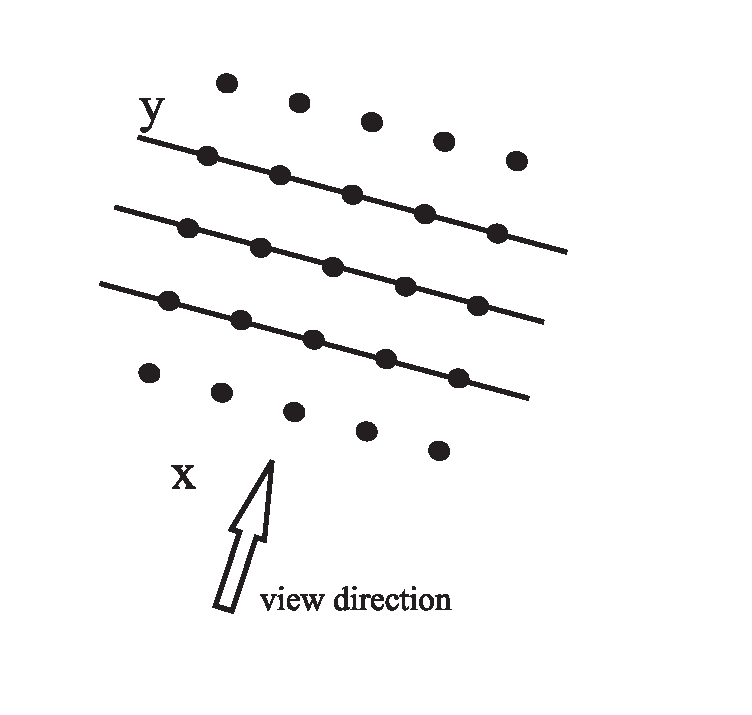
\includegraphics[width=2.0in]{figurest/figDIRA2}&
\includegraphics[width=2.0in]{figurest/figDIRA3}&
\includegraphics[width=2.0in]{figurest/figDIRA1}\\
a) smoke planes parallel to $y$ axis& b) smoke planes parallel to
$y=x$ axis)&
c) smoke planes parallel to $x$ axis\\
\end{tabular}
\caption{View of smoke planes from above.  Smoke Planes are
oriented so that are ``most perpendicular'' to the line of sight }
\label{figDIRA}
\end{figure}

\begin{figure}
\centerline{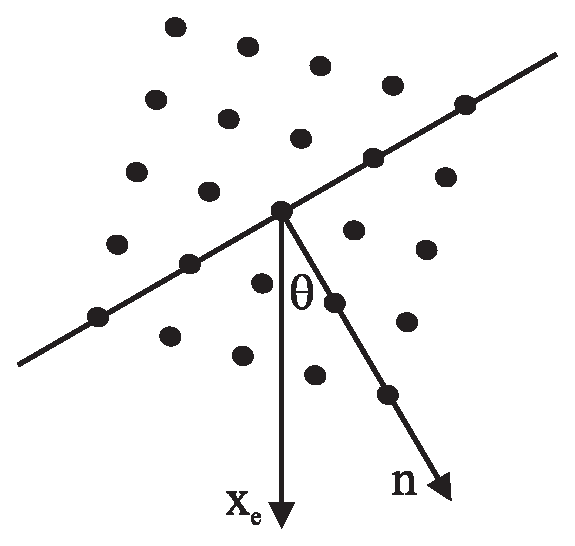
\includegraphics[width=3.0in]{figurest/figDIRB}}
\caption{Diagram illustrating the angle between the line of sight
and smoke plane normal vector.  View planes are chosen to minimize
this angle.} \label{figDIRB}
\end{figure}
Figure \ref{figDIRA} illustrates three directions from which to
view smoke planes.  Another three view directions occur on the
back side of these planes.  In order to minimize off-axis viewing,
a set of view planes are selected so that the angle between the
candidate smoke plane normal vector and the view direction is
minimized.

This angle, $\theta$, illustrated in Figure \ref{figDIRB},
satifies
\begin{eqnarray*}
\cos(\theta)=\frac{n\cdot v_e}{||n||||v_e||}
\end{eqnarray*}

where $n$ is the candidate smoke plane normal vector and $v_e$ is
the view direction vector.  In OpenGL, the view direction vector,
$v_e$, is computed by simply obtaining the modelview matrix, $M$
and multiplying it by the vector, $(0,0,1)^T$ or equivalently the
third row of the $M$.


\subsubsection{Blending, Drawing Transparent Objects} OpenGL allows
one to draw a series of triangles specifying the location and
color of each node.  The color is specified as a quadruple of red,
green, blue and alpha value each ranging from zero to one.  The
quantity, $1-\alpha$ represents a transparency or the fraction of
the scene that shows through or blends with this region.

The $\alpha$'s can then be used to represent smoke.
